% physicskit: a verified toolkit for computational physics, across its domains
%
% Draft for SciPost Physics Codebases. Written with the standard article
% class: move the body into SciPost's template (SciPost.cls) before
% submission. Figures and tables come from paper/figures/build_all.py.
\documentclass[11pt,a4paper]{article}

\usepackage[margin=2.5cm]{geometry}
\usepackage{amsmath,amssymb}
\usepackage{graphicx}
\usepackage{booktabs}
\usepackage{tabularx}
\usepackage{siunitx}
\usepackage{xcolor}
\usepackage{listings}
\usepackage{hyperref}
\usepackage{tikz}
\usetikzlibrary{arrows.meta,positioning,fit}

\lstset{language=Python, basicstyle=\ttfamily\footnotesize, columns=fullflexible,
        keywordstyle=\color{blue!60!black}, commentstyle=\color{gray}, frame=lines,
        breaklines=true, showstringspaces=false}
\newcommand{\code}[1]{\texttt{#1}}
% table rows from paper/figures/build_all.py (the primitive \input is safe inside tabular)
\makeatletter\newcommand{\rows}[1]{\@@input #1.tex }\makeatother
\graphicspath{{figures/}}
\newcommand{\physicskitversion}{0.4.0}
\newcommand{\qutipversion}{5.3.1}
\newcommand{\astropyversion}{8.0.1}
\newcommand{\numpyversion}{2.5.3}
\newcommand{\scipyversion}{1.18.1}
\newcommand{\numbaversion}{0.68.0}

\IfFileExists{tables/bench_setup.tex}{\newcommand{\benchplatform}{macOS-26.6.2-arm64-arm-64bit}
}{}

\title{physicskit: a verified Python toolkit for computational physics,\\
       from classical chaos to black holes}
\author{Charles Poli\thanks{\href{mailto:cpoli374@gmail.com}{cpoli374@gmail.com}}}
\date{Codebase release \physicskitversion}

\begin{document}
\maketitle

\begin{abstract}
physicskit is an open-source Python package for learning, teaching and
exploring computational physics across fourteen domains: classical
mechanics, chaos, quantum and semiclassical mechanics, condensed matter,
statistical physics, fields and optics, fluids, plasmas, general relativity,
astrophysics, particle physics and random matrix theory. It is built on
NumPy and SciPy, with numba-compiled time-stepping loops, a shared layer of
ODE and SDE integrators, and one API convention across the domains. Every
simulation keeps its full trajectory, and every domain ships plotting and
animation helpers. The package is built around verification. Its 2247 unit
tests prefer closed forms to snapshots, its docstring examples run in
continuous integration, and each of its 392 gallery examples asserts the
result it illustrates before plotting it, so that the documentation states
nothing that the code does not check on every commit. The gallery is
organized by history: each domain's documentation tells its field as a
chronology of breakthroughs, each linked to the examples that reproduce
it. We describe the design, survey the domains, follow one potential, $-1/r$,
from Kepler's ellipse to hydrogen's levels across four subpackages, and
validate physicskit against QuTiP~\cite{johansson2012,lambert2024},
Astropy~\cite{astropy2022} and SciPy~\cite{virtanen2020}. The three
independent packages agree with physicskit to within $5\times10^{-12}$
on states, spectra, Wigner functions, open-system dynamics and cosmological
distances, and to the integration tolerance where a tolerance applies. We
also benchmark physicskit against them and state where each one is the
better choice.
\end{abstract}

\tableofcontents

%----------------------------------------------------------------------------
\section{Introduction}
\label{sec:intro}

Computational physics is taught as one subject but practised in many
packages. Mature, specialized codes serve each field: QuTiP for open
quantum systems~\cite{johansson2012,lambert2024}, Astropy for
astronomy~\cite{astropy2022}, Kwant for quantum transport~\cite{groth2014},
Dedalus for spectral fluid dynamics~\cite{burns2020}, and many more. They
are built for research at scale, and each has its own data model, units
and conventions. Textbooks of computational physics~\cite{newman2013,landau2015}
cover the breadth instead, with short programs that a student writes and
then discards.

Between the two sits a gap that a student or an instructor meets quickly.
A course that runs from the Kepler problem to the Lorenz attractor, the
hydrogen atom, the Ising model and a black hole's shadow needs either
several research packages, each with its own learning curve, or a pile of
one-off scripts whose correctness nobody checks. Neither shows that the
same few numerical ideas (a symplectic step, a sparse eigensolver, a fast
Fourier transform, a Monte Carlo update) recur across the fields.

physicskit addresses this with one package and one convention across
fourteen domains (Sec.~\ref{sec:design}). We do not claim it is the
fastest or the most complete package for any one field: QuTiP, Astropy and
the other specialized codes scale further and cover more within their
domains, and we measure where (Sec.~\ref{sec:performance}). What physicskit
provides is breadth in one package, with algorithms a reader can inspect,
and verification throughout. Every numerical claim of its gallery is
asserted by code that runs in continuous integration (CI), and its results
agree with QuTiP, Astropy and SciPy to near machine precision
(Sec.~\ref{sec:validation}).

This paper is organized as a user guide. Section~\ref{sec:design}
describes the design. Sections~\ref{sec:mechanics} to~\ref{sec:particles}
survey the domains, two at a time, and Sec.~\ref{sec:example} follows one
problem across four of them. Section~\ref{sec:validation} validates the
results, Sec.~\ref{sec:performance} measures performance, and
Sec.~\ref{sec:teaching} describes the gallery and the history pages as
teaching material.

%----------------------------------------------------------------------------
\section{Design}
\label{sec:design}

\begin{figure}[t]
\centering
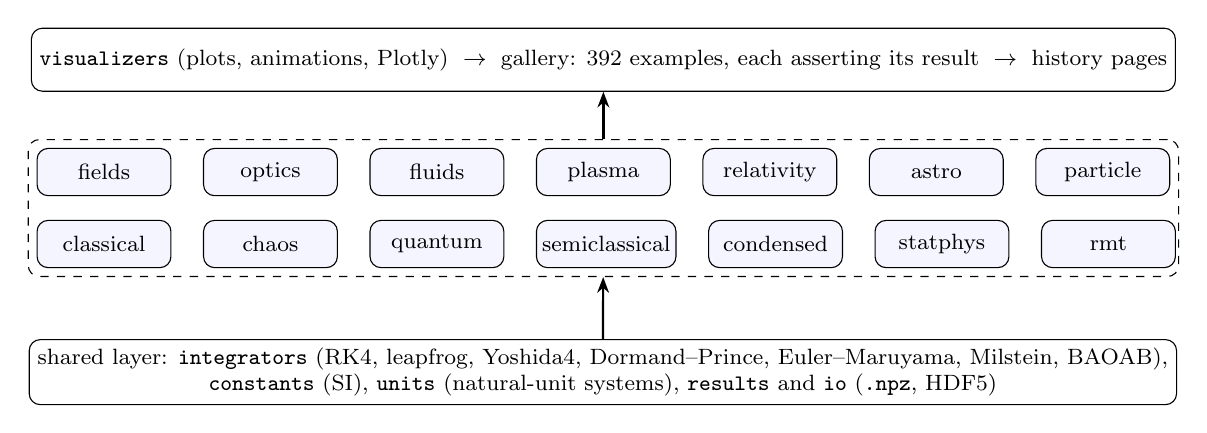
\begin{tikzpicture}[node distance=5mm and 4mm, every node/.style={font=\footnotesize},
  box/.style={draw, rounded corners, align=center, minimum height=8mm, inner sep=3pt},
  dom/.style={draw, rounded corners, align=center, minimum height=6mm, minimum width=17mm, inner sep=2pt, fill=blue!4},
  arr/.style={-{Stealth[length=2mm]}, thick}]
\node[box, minimum width=14.5cm] (shared) {shared layer: \code{integrators} (RK4, leapfrog, Yoshida4, Dormand--Prince, Euler--Maruyama, Milstein, BAOAB),\\ \code{constants} (SI), \code{units} (natural-unit systems), \code{results} and \code{io} (\code{.npz}, HDF5)};
\node[dom, above=9mm of shared.north west, anchor=south west, xshift=1mm] (d1) {classical};
\node[dom, right=of d1] (d2) {chaos};
\node[dom, right=of d2] (d3) {quantum};
\node[dom, right=of d3] (d4) {semiclassical};
\node[dom, right=of d4] (d5) {condensed};
\node[dom, right=of d5] (d6) {statphys};
\node[dom, right=of d6] (d7) {rmt};
\node[dom, above=3mm of d1] (e1) {fields};
\node[dom, right=of e1] (e2) {optics};
\node[dom, right=of e2] (e3) {fluids};
\node[dom, right=of e3] (e4) {plasma};
\node[dom, right=of e4] (e5) {relativity};
\node[dom, right=of e5] (e6) {astro};
\node[dom, right=of e6] (e7) {particle};
\node[draw, dashed, rounded corners, inner sep=3pt, fit=(d1)(e7)] (domains) {};
\node[box, above=6mm of domains, minimum width=14.5cm] (docs) {\code{visualizers} (plots, animations, Plotly) $\;\to\;$ gallery: 392 examples, each asserting its result $\;\to\;$ history pages};
\draw[arr] (shared) -- (domains);
\draw[arr] (domains) -- (docs);
\end{tikzpicture}
\caption{The layers of physicskit. Fourteen domain subpackages share one
layer of integrators, constants, unit systems and result containers. Each
domain has its own plotting and animation helpers, which the gallery
examples use; the history pages of the documentation link every
breakthrough of a field to the examples that reproduce it.}
\label{fig:design}
\end{figure}

\paragraph{One subpackage per domain.} Each of the fourteen domains is a
subpackage, \code{physicskit.<domain>}, with its own tests beside it
(Fig.~\ref{fig:design}). Small domains are flat modules; larger ones split
into \code{core} (base classes, integrators), \code{systems} or
\code{chapters} (concrete models), \code{utils} and \code{visualizers}.
The package is imported as \code{pk}, and every domain is reached as an
attribute, \code{pk.chaos}, \code{pk.relativity} and so on. Its runtime
dependencies are NumPy~\cite{harris2020}, SciPy~\cite{virtanen2020},
matplotlib~\cite{hunter2007}, numba~\cite{lam2015}, SymPy~\cite{meurer2017},
Plotly and tqdm.

\paragraph{Library first, hand-rolled where the steps are the lesson.}
physicskit calls NumPy and SciPy for everything they implement: fast
Fourier transforms, dense and sparse eigensolvers, quadrature, special
functions and statistical tests. It writes an algorithm itself only where
the algorithm's steps are the subject being taught, as for symplectic
integrators~\cite{yoshida1990}, the Boris pusher~\cite{boris1970},
particle-in-cell~\cite{birdsall1991}, the Yee scheme~\cite{yee1966},
Metropolis and Wolff updates~\cite{metropolis1953,wolff1989} and geodesic
ray tracing, or where no library equivalent exists, as for topological
invariants and billiard maps.

\paragraph{Shared integrators and the numba pattern.} The shared
integrators (\code{pk.integrators}) are numba-compiled and take a
right-hand side \code{f(state, t, params)}. A compiled step loop can only
call a compiled callback, so every concrete system builds a standalone
\code{@njit} force or derivative function from a module-level factory that
closes over its parameters, and the base classes integrate with it. The
convention lets one compiled callback serve every parameter value, and it
keeps the time-stepping loops of \code{chaos}, \code{classical},
\code{fluids}, \code{plasma}, \code{relativity} and \code{statphys} in
compiled code. A few domains keep their own integrators where the physics
asks for it, such as the periodic-boundary, force-caching molecular
dynamics engine of \code{statphys}; these divergences are documented.

\paragraph{Trajectories and units.} Every \code{integrate()} or
\code{simulate()} call returns the whole trajectory (times, states and the
conserved quantities of the system), not only its end point, so a student
can plot energy drift or a Poincar\'e section from the same call. Each
domain computes in its field's natural units: $G=1$ in \code{astro},
$G=c=1$ in \code{relativity}, $\hbar=1$ in \code{quantum}, $k_B=1$ in
\code{statphys}. \code{pk.constants} holds the SI values (CODATA, through
\code{scipy.constants}), and \code{pk.units} builds explicit natural-unit
systems with user-chosen scales and converts them to SI. A shared
\code{Result} container, saved to \code{.npz} or HDF5, carries units with
the data.

\paragraph{Verification policy.} The test suite (2247 tests) runs on
Python 3.10--3.15, on Linux and macOS. Tests assert closed forms and
analytically verifiable quantities (\code{pytest.approx} against a known
formula) rather than snapshots of plots; a visualizer gets a smoke test of
its return type or of its saved animation. Every public function has a
NumPy-style docstring, whose examples run as doctests in CI. Every new
formula cites its source, so that it can be checked independently. The
whole package type-checks with mypy, which CI enforces. The 392 gallery
examples are executed by every documentation build, which CI runs on each
push, and each ends with a cell of assertions against the closed form or
known value it illustrates. A change that breaks the physics of an example
therefore fails CI. Section~\ref{sec:validation} adds independent checks
against QuTiP, Astropy and SciPy.

%----------------------------------------------------------------------------
\section{Classical mechanics and chaos}
\label{sec:mechanics}

\begin{figure}[t]
\centering
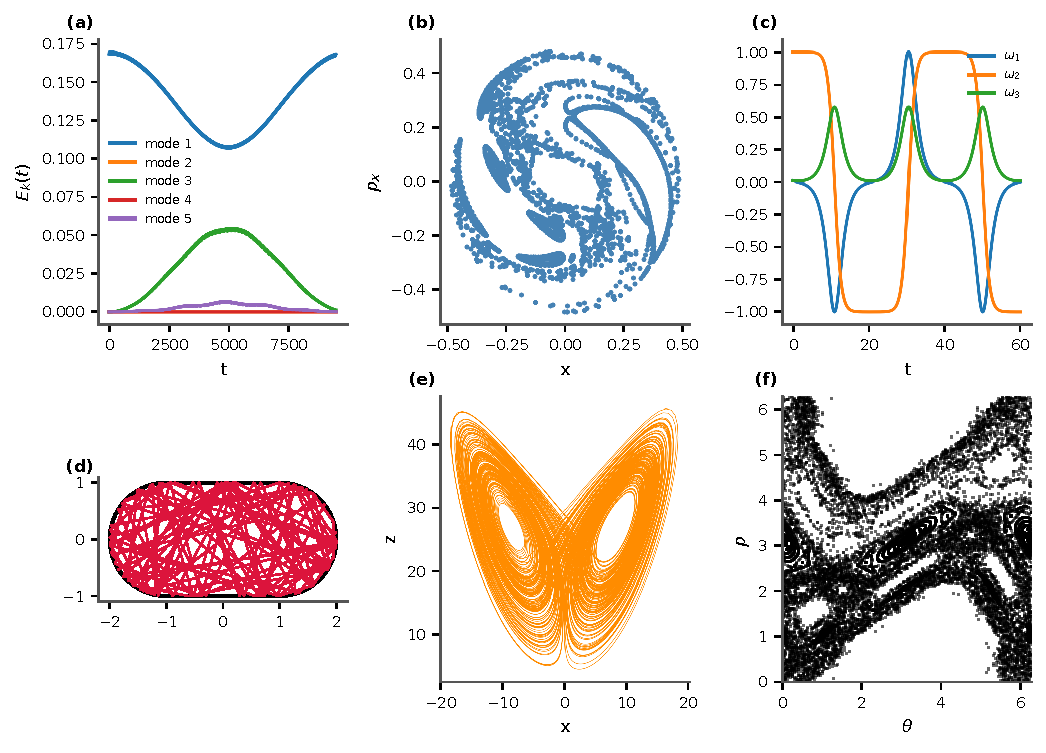
\includegraphics[width=\textwidth]{fig_mechanics}
\caption{Classical mechanics (top) and chaos (bottom). (a)~The
Fermi--Pasta--Ulam--Tsingou recurrence: the energy of the first normal
mode leaves and returns. (b)~Poincar\'e section of the H\'enon--Heiles
system, with KAM tori broken into a chaotic sea. (c)~The Dzhanibekov
effect: a body spinning about its intermediate axis flips periodically.
(d)~A chaotic trajectory in the Bunimovich stadium. (e)~The Lorenz
attractor. (f)~Chirikov's standard map: KAM islands in a chaotic sea.}
\label{fig:mechanics}
\end{figure}

\paragraph{Classical.} \code{pk.classical} builds Newtonian, Lagrangian and
Hamiltonian systems on the shared integrators. A symbolic engine derives
the equations of motion from a Lagrangian $L = T - V$ written in SymPy and
compiles them, so a new mechanical system takes a few lines. Lattice
dynamics reproduces the FPUT recurrence~\cite{fermi1955}
[Fig.~\ref{fig:mechanics}(a)] and sine-Gordon kinks; Hamiltonian systems
give Poincar\'e sections and KAM tori~\cite{henon1964}
[Fig.~\ref{fig:mechanics}(b)]; rigid bodies, with an implicit-midpoint
integrator that conserves energy and angular momentum to round-off, show
the Dzhanibekov effect [Fig.~\ref{fig:mechanics}(c)], the heavy top,
Euler's disk and the rattleback. A timestep estimator picks the step that
reaches a requested energy drift.

\paragraph{Chaos.} \code{pk.chaos} holds continuous flows (Lorenz~\cite{lorenz1963},
R\"ossler, Duffing, Chua, the double and magnetic pendulums), discrete maps
(logistic, H\'enon, standard~\cite{chirikov1979}, baker's, the Smale
horseshoe) and billiards (circle, ellipse, stadium~\cite{bunimovich1979},
Sinai) [Fig.~\ref{fig:mechanics}(d)--(f)]. Diagnostics include the full
Lyapunov spectrum by Benettin's QR method~\cite{benettin1980}, box-counting
and correlation dimensions, recurrence plots, bifurcation diagrams and
basins of attraction. Its \code{quantum} module quantizes billiards (a
finite-difference Laplacian solved by shift-invert Lanczos) and maps (the
quantum kicked rotor and baker's map), with Husimi functions, and so leads
into the semiclassical and random-matrix domains.

%----------------------------------------------------------------------------
\section{Quantum and semiclassical mechanics}
\label{sec:quantum}

\begin{figure}[t]
\centering
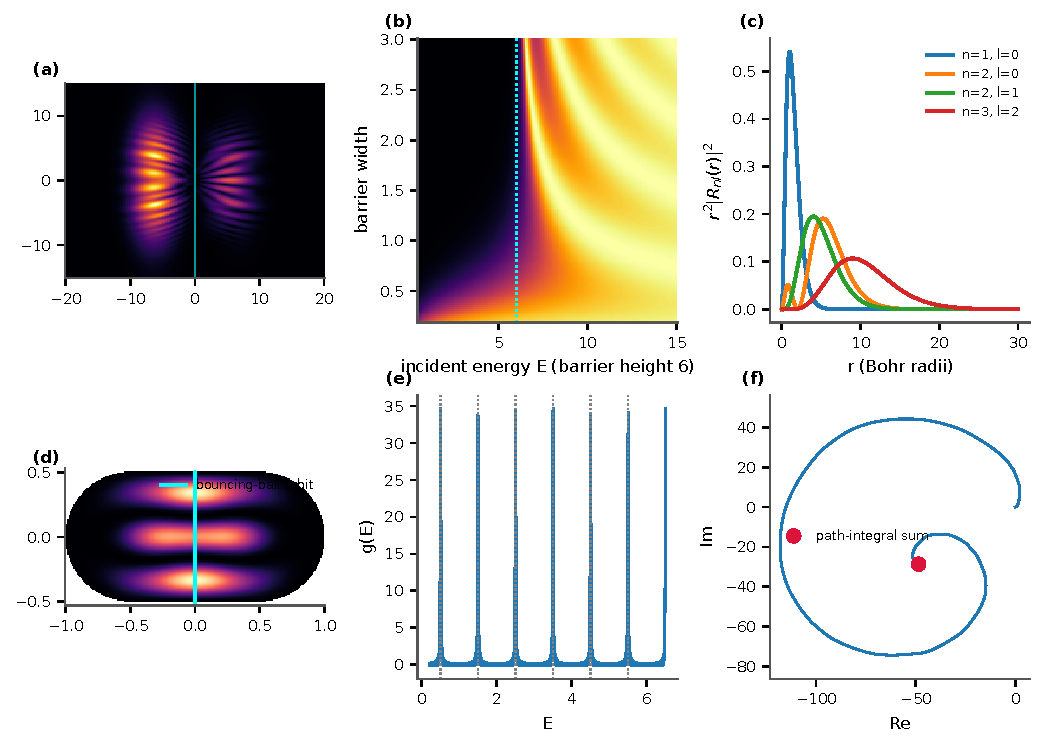
\includegraphics[width=\textwidth]{fig_quantum}
\caption{Quantum (top) and semiclassical (bottom) mechanics. (a)~A wave
packet through a double slit, split-operator propagation. (b)~Transmission
through a barrier against energy and width, with its resonances above the
barrier. (c)~Radial probability densities of hydrogen. (d)~An eigenstate
of the stadium scarred by the bouncing-ball orbit. (e)~The Gutzwiller trace
formula: a level density rebuilt from classical periodic orbits.
(f)~Feynman's sum over paths: the phasor spiral of the path integral.}
\label{fig:quantum}
\end{figure}

\paragraph{Quantum.} \code{pk.quantum} propagates wave packets in one and
two dimensions with the split-operator method~\cite{feit1982}
[Fig.~\ref{fig:quantum}(a)], and finds bound states with a matrix Numerov
solver and sparse eigensolvers [Fig.~\ref{fig:quantum}(b)]. It covers
hydrogen and angular momentum [Fig.~\ref{fig:quantum}(c)], spin and the
Bloch sphere, entanglement and Bell inequalities, measurement,
perturbation and Floquet theory, the Dirac and Klein--Gordon equations,
Born and partial-wave scattering, Hartree--Fock for small atoms and
molecules, quantum circuits (Deutsch--Jozsa, Grover, Shor's period
finding), and matrix-product states evolved by TEBD~\cite{vidal2003}. Open
systems are treated three ways that cross-check each other: the Lindblad
equation~\cite{lindblad1976} through the exponential of its Liouvillian,
Kraus maps, and quantum trajectories~\cite{dalibard1992}.

\paragraph{Semiclassical.} \code{pk.semiclassical} connects classical
orbits to quantum spectra. It implements WKB and EBK quantization with
Maslov indices and the Langer correction~\cite{langer1937}; the Van Vleck,
Herman--Kluk~\cite{herman1984} and thawed-Gaussian propagators; Feynman's
path integral~\cite{feynman1948} [Fig.~\ref{fig:quantum}(f)]; the
Gutzwiller~\cite{gutzwiller1971} and Berry--Tabor trace formulas
[Fig.~\ref{fig:quantum}(e)]; Bogomolny's transfer operator; and quantum
scars~\cite{heller1984} [Fig.~\ref{fig:quantum}(d)].

%----------------------------------------------------------------------------
\section{Condensed matter and statistical physics}
\label{sec:matter}

\begin{figure}[t]
\centering
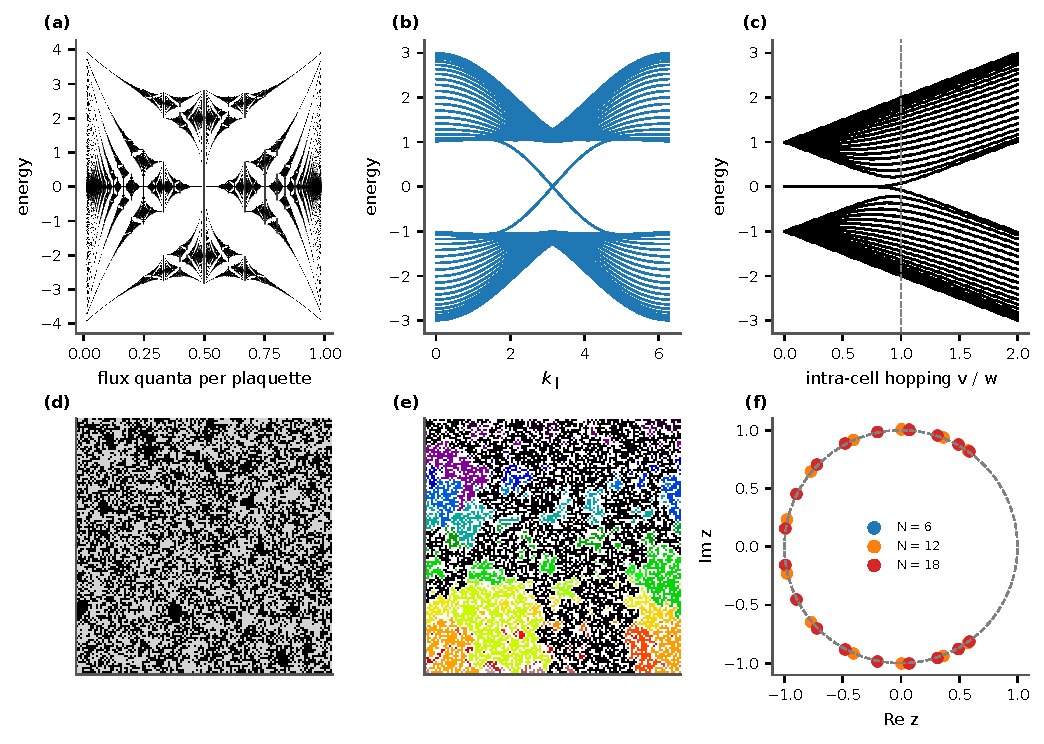
\includegraphics[width=\textwidth]{fig_matter}
\caption{Condensed matter (top) and statistical physics (bottom). (a)~The
Hofstadter butterfly. (b)~Chiral edge states of a Haldane-model ribbon
cross the bulk gap. (c)~Spectrum of a finite SSH chain against the
hopping ratio: zero-energy edge modes for $v < w$. (d)~The 2D Ising model
at its critical temperature. (e)~Site-percolation clusters at the
threshold. (f)~Lee--Yang zeros of finite Ising rings on the unit circle.}
\label{fig:matter}
\end{figure}

\paragraph{Condensed matter.} \code{pk.condensed} builds Bloch Hamiltonians,
Slater--Koster models and Peierls phases, which give the Hofstadter
butterfly~\cite{hofstadter1976} [Fig.~\ref{fig:matter}(a)]. Its topology
tools compute Chern numbers~\cite{thouless1982}, Zak phases and
$\mathbb{Z}_2$ invariants, classify Hamiltonians in the tenfold way, and
cut ribbons and flakes to show edge states of the SSH~\cite{su1979},
Haldane~\cite{haldane1988}, Kane--Mele, Kitaev and Weyl models
[Fig.~\ref{fig:matter}(b,c)]. It covers Anderson localization, Landau
levels and the quantum Hall effects, BCS, Hubbard and Ginzburg--Landau
theory, phonons and the Debye heat capacity, and Drude and Boltzmann
transport. Spin chains are diagonalized exactly in sparse symmetry sectors
and compared with the Bethe ansatz~\cite{bethe1931} and with free fermions.
For tight-binding models beyond this scope, a companion package,
tbkit~\cite{tbkit}, adds quantum transport, finite lattices with defects
and the kernel polynomial method.

\paragraph{Statistical physics.} \code{pk.statphys} samples Ising, Potts and
XY models with numba-compiled Metropolis and Wolff
updates~\cite{metropolis1953,wolff1989}, and compares them with Onsager's
exact solution~\cite{onsager1944} [Fig.~\ref{fig:matter}(d)]. It covers
finite-size scaling and block-spin renormalization, percolation
[Fig.~\ref{fig:matter}(e)], self-organized criticality, KPZ
growth~\cite{kardar1986}, spin glasses, Wang--Landau sampling, path-integral
Monte Carlo, Lee--Yang zeros~\cite{lee1952} [Fig.~\ref{fig:matter}(f)],
molecular dynamics, Jarzynski's equality~\cite{jarzynski1997}, and
Langevin, Ornstein--Uhlenbeck and Fokker--Planck dynamics on the shared
stochastic integrators.

%----------------------------------------------------------------------------
\section{Fields and optics}
\label{sec:waves}

\begin{figure}[t]
\centering
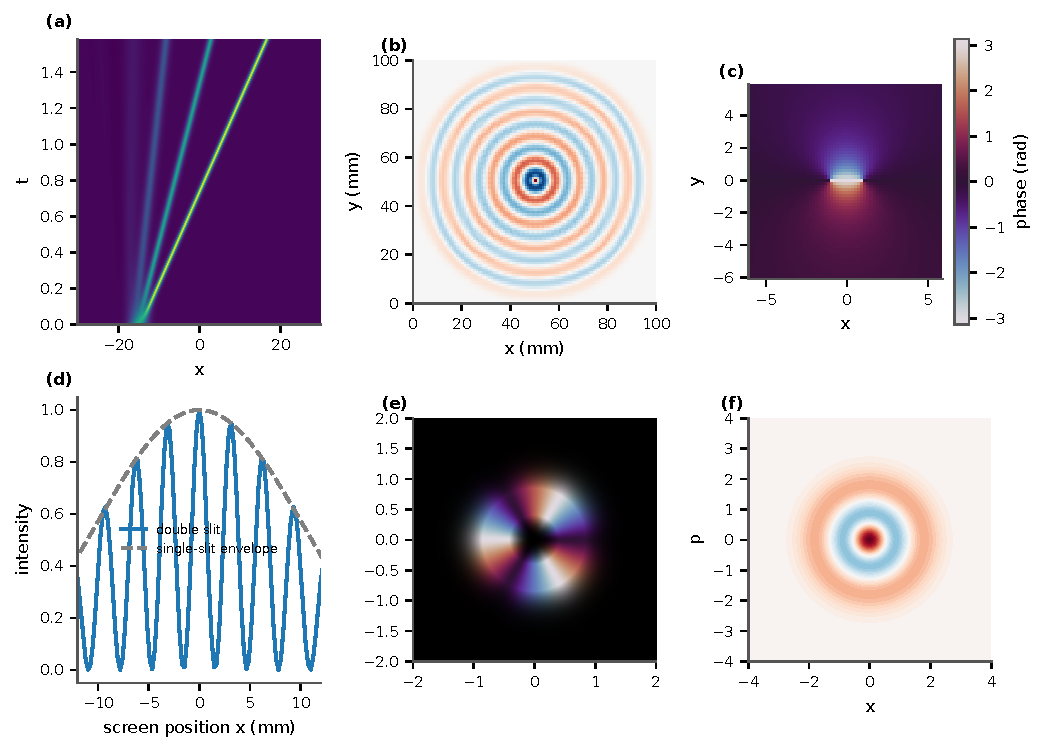
\includegraphics[width=\textwidth]{fig_waves}
\caption{Fields (top) and optics (bottom). (a)~A KdV bump fissions into a
train of solitons. (b)~A dipole radiating on the Yee grid (FDTD).
(c)~Phase of a Bose--Einstein condensate holding a vortex--antivortex pair.
(d)~Young's double-slit fringes under their single-slit envelope. (e)~A
Laguerre--Gauss vortex beam, $l = 3$. (f)~The Wigner function of the Fock
state $|2\rangle$, negative in places.}
\label{fig:waves}
\end{figure}

\paragraph{Fields.} \code{pk.fields} solves electrostatics (Poisson
relaxation, the method of images, multipole expansions) and Biot--Savart
magnetostatics, and propagates Maxwell's equations by FDTD on the Yee
grid~\cite{yee1966} with perfectly matched layers~\cite{berenger1994}
[Fig.~\ref{fig:waves}(b)]. Split-step spectral solvers integrate the KdV,
nonlinear Schr\"odinger and sine-Gordon equations~\cite{zabusky1965}
[Fig.~\ref{fig:waves}(a)], and the Gross--Pitaevskii equation, in real and
imaginary time, gives condensate ground states, quantized vortices and
vortex lattices [Fig.~\ref{fig:waves}(c)].

\paragraph{Optics.} \code{pk.optics} covers ray optics and ABCD matrices,
Fresnel and Fraunhofer diffraction by FFT [Fig.~\ref{fig:waves}(d)],
Gaussian and Laguerre--Gauss beams~\cite{allen1992}
[Fig.~\ref{fig:waves}(e)], thin films and photonic band gaps, nonlinear
optics and phase matching, and lasers from rate equations to Maxwell--Bloch
chaos. Its quantum optics works in a truncated Fock basis: coherent and
squeezed states, photon statistics, Wigner functions from their closed-form
Fock matrix elements~\cite{cahill1969} [Fig.~\ref{fig:waves}(f)], and the
Jaynes--Cummings model~\cite{jaynes1963}.

%----------------------------------------------------------------------------
\section{Fluids and plasmas}
\label{sec:flows}

\begin{figure}[t]
\centering
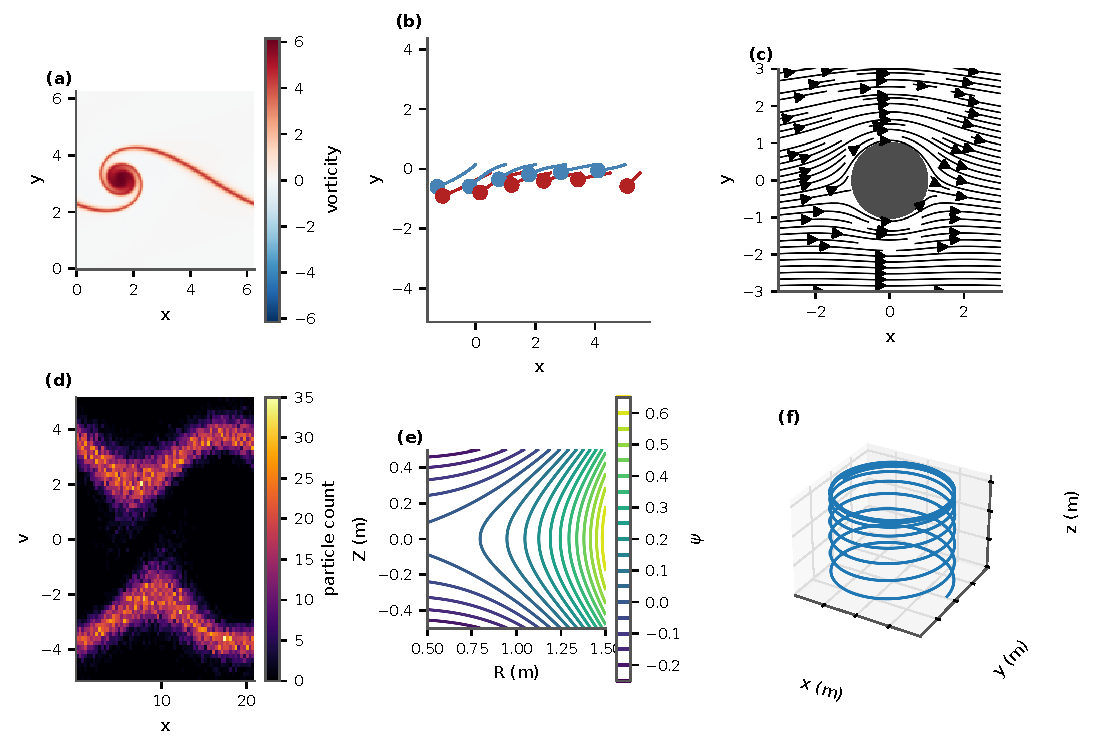
\includegraphics[width=\textwidth]{fig_flows}
\caption{Fluids (top) and plasmas (bottom). (a)~Kelvin--Helmholtz roll-up
of a shear layer (vorticity). (b)~A von K\'arm\'an street of point vortices
drifting as a whole. (c)~Potential flow past a spinning cylinder, whose
circulation produces Kutta--Joukowski lift. (d)~Phase space of the
two-stream instability: a vortex in a particle-in-cell simulation.
(e)~Nested flux surfaces of a Grad--Shafranov equilibrium. (f)~A proton
bouncing in a magnetic mirror.}
\label{fig:flows}
\end{figure}

\paragraph{Fluids.} \code{pk.fluids} solves the 2D incompressible
Navier--Stokes equations pseudo-spectrally, which give the
Kelvin--Helmholtz and Rayleigh--Taylor instabilities
[Fig.~\ref{fig:flows}(a)] and forced turbulence with Kolmogorov's
cascade~\cite{kolmogorov1941}. It also holds potential flow and the
Kutta--Joukowski lift [Fig.~\ref{fig:flows}(c)], viscous exact solutions
(Couette, Poiseuille, Blasius, Stokes drag), point-vortex dynamics
[Fig.~\ref{fig:flows}(b)], compressible shocks and the Sod
tube~\cite{sod1978}, shallow water, Rayleigh--B\'enard onset, linear
elasticity by finite elements, and a D2Q9 lattice Boltzmann
solver~\cite{qian1992}.

\paragraph{Plasmas.} \code{pk.plasma} pushes particles with the Boris
scheme~\cite{boris1970} through guiding-centre drifts and magnetic mirrors
[Fig.~\ref{fig:flows}(f)]; solves the Grad--Shafranov
equation~\cite{shafranov1966} for tokamak equilibria
[Fig.~\ref{fig:flows}(e)]; gives cold-plasma dispersion and the CMA
diagram; and runs electrostatic particle-in-cell
simulations~\cite{birdsall1991} of Landau damping~\cite{landau1946}, the
two-stream [Fig.~\ref{fig:flows}(d)] and Weibel instabilities. It also
covers magnetic reconnection and Hasegawa--Mima drift-wave
turbulence~\cite{hasegawa1978}.

%----------------------------------------------------------------------------
\section{Gravitation and astrophysics}
\label{sec:cosmos}

\begin{figure}[t]
\centering
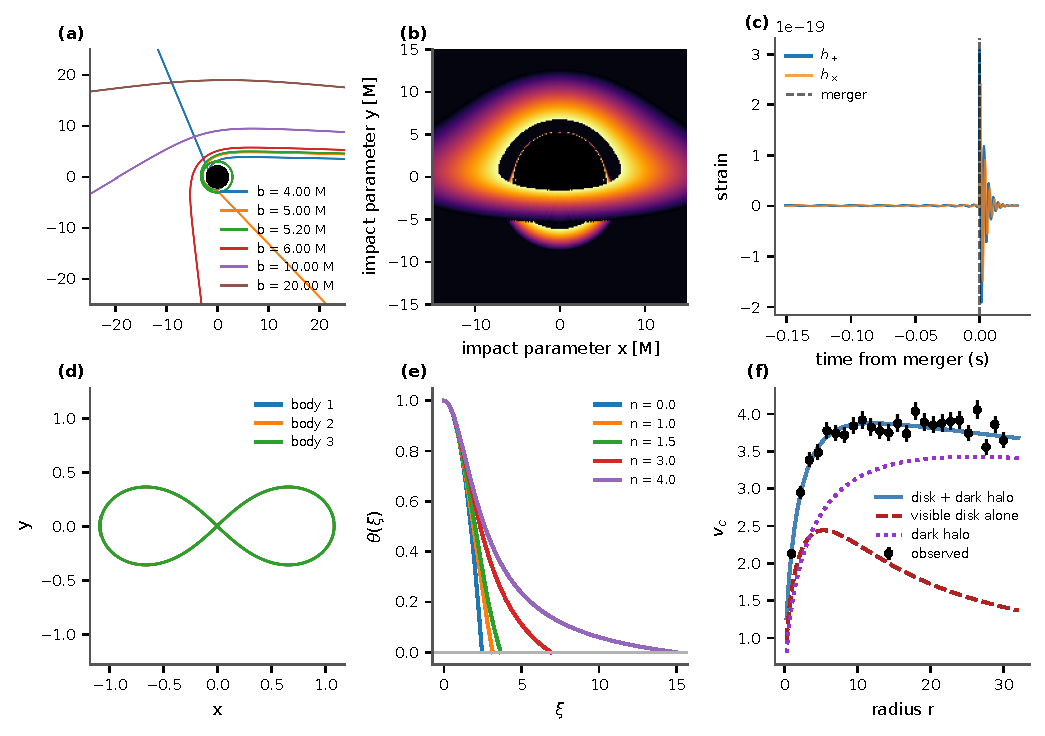
\includegraphics[width=\textwidth]{fig_cosmos}
\caption{General relativity (top) and astrophysics (bottom). (a)~Null
geodesics bending around a Schwarzschild black hole, for several impact
parameters. (b)~A ray-traced black-hole shadow with its accretion disk.
(c)~The GW150914 chirp, from inspiral to merger and ringdown. (d)~The
figure-eight three-body choreography. (e)~Lane--Emden polytropes. (f)~A
flat galactic rotation curve: a visible disk alone falls off, a dark halo
holds it flat.}
\label{fig:cosmos}
\end{figure}

\paragraph{Relativity.} \code{pk.relativity} integrates timelike and null
geodesics of the Schwarzschild, Kerr~\cite{kerr1963} and Kerr--Newman
metrics in compiled code [Fig.~\ref{fig:cosmos}(a)], and ray-traces black
hole shadows and accretion disks [Fig.~\ref{fig:cosmos}(b)]. It covers
gravitational lensing, gravitational waves from the quadrupole formula and
Peters' orbital decay~\cite{peters1964} to a leading-order
inspiral--merger--ringdown waveform [Fig.~\ref{fig:cosmos}(c)]~\cite{abbott2016}, neutron stars from
the TOV equations~\cite{oppenheimer1939}, FLRW cosmology, and ADM initial
data~\cite{arnowitt1959}. A numerical curvature engine computes Christoffel
symbols, Riemann and Einstein tensors of any metric by finite
differences, and is validated against Einstein's vacuum field equations.

\paragraph{Astrophysics.} \code{pk.astro} integrates $N$-body systems with
symplectic schemes, including the figure-eight
choreography~\cite{chenciner2000} [Fig.~\ref{fig:cosmos}(d)]; solves stellar
structure from Lane--Emden polytropes [Fig.~\ref{fig:cosmos}(e)] to the
Chandrasekhar mass; and covers Keplerian orbits and Hohmann transfers,
galactic rotation curves with NFW halos~\cite{navarro1996}
[Fig.~\ref{fig:cosmos}(f)], grey radiative transfer, smoothed-particle
hydrodynamics, Zel'dovich's cosmic web~\cite{zeldovich1970}, and stellar
convection with an $\alpha$--$\Omega$ dynamo.

%----------------------------------------------------------------------------
\section{Particles and random matrices}
\label{sec:particles}

\begin{figure}[t]
\centering
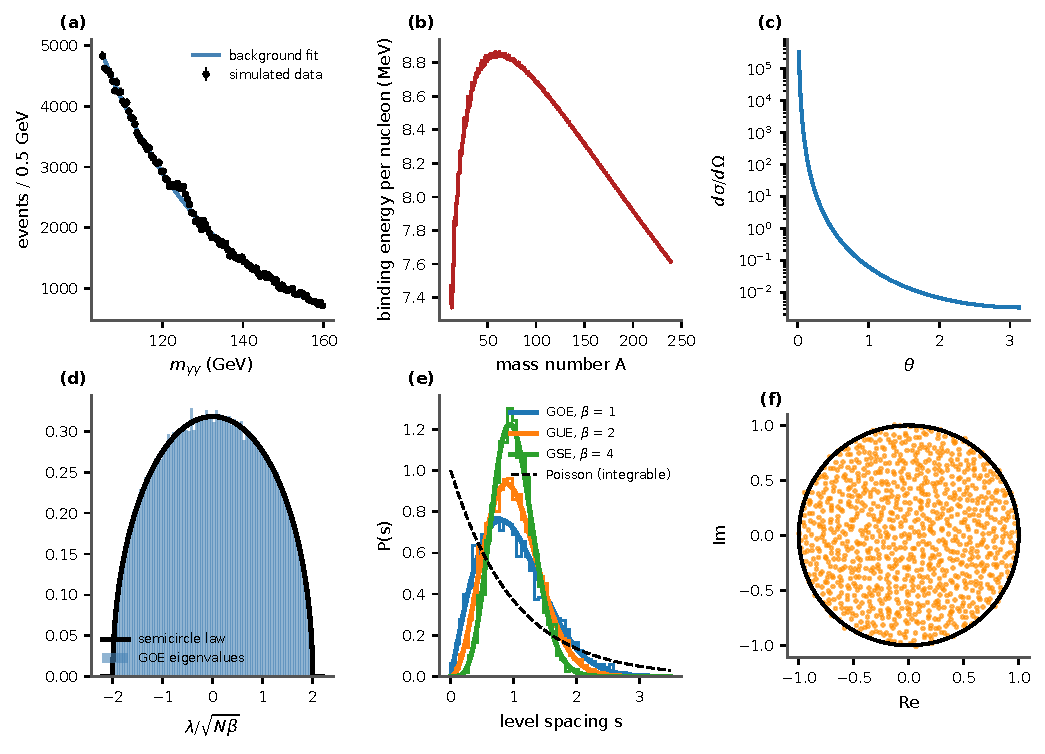
\includegraphics[width=\textwidth]{fig_particles}
\caption{Particle physics (top) and random matrix theory (bottom). (a)~A
simulated $H\to\gamma\gamma$ search: a bump over a falling background.
(b)~Binding energy per nucleon from Weizs\"acker's semi-empirical mass
formula. (c)~The Rutherford cross section. (d)~Wigner's semicircle law.
(e)~Level-spacing distributions of the three Gaussian ensembles, against
Poisson. (f)~Ginibre's circular law.}
\label{fig:particles}
\end{figure}

\paragraph{Particle physics.} \code{pk.particle} provides four-vectors,
boosts and Mandelstam variables; two- and three-body decays and scattering
cross sections; detector signatures and simulated resonance searches from
the $J/\psi$ to the Higgs boson~\cite{atlas2012} [Fig.~\ref{fig:particles}(a)];
weak interactions, CP violation and neutrino oscillations; radioactive
decay chains; nuclear physics from Rutherford scattering~\cite{rutherford1911}
to the semi-empirical mass formula~\cite{weizsacker1935} and fission
[Fig.~\ref{fig:particles}(b,c)]; and U(1) lattice gauge theory with Wilson
loops~\cite{wilson1974}.

\paragraph{Random matrix theory.} \code{pk.rmt} is organized around Dyson's
threefold way~\cite{dyson1962}. It samples Gaussian, circular, Ginibre,
Wishart, Jacobi and Bogoliubov--de Gennes ensembles, with tridiagonal
$\beta$-ensembles~\cite{dumitriu2002} for large sizes, and validates each
classic law against its closed form with Kolmogorov--Smirnov tests: the
semicircle~\cite{wigner1955}, the Wigner surmise, Tracy--Widom~\cite{tracy1994},
Marchenko--Pastur and the circular law~\cite{ginibre1965}
[Fig.~\ref{fig:particles}(d)--(f)]. It connects back to quantum chaos
through the Bohigas--Giannoni--Schmit conjecture~\cite{bohigas1984}.

%----------------------------------------------------------------------------
\section{A worked example: one potential across four subpackages}
\label{sec:example}

Listing~\ref{lst:kepler} follows one potential, $-1/r$, through four
subpackages and the shared integrators. The listing is the file
\code{paper/listings/inverse\_square\_workflow.py} of the repository, which
the paper's validation runs, so the code printed here is code that passes.

\lstinputlisting[caption={The potential $-1/r$ from Kepler's ellipse to
hydrogen's levels. Every step asserts its result.}, label=lst:kepler,
firstline=2]{../listings/inverse_square_workflow.py}

Step~1 builds an ellipse from its orbital elements (\code{astro}) and
integrates it for one Kepler period with the shared fourth-order symplectic
integrator: the orbit closes and the energy is conserved to $10^{-9}$.
Step~2 replaces Newton by Einstein (\code{relativity}): a Schwarzschild
geodesic at $r\sim 20M$ no longer closes, and its periapsis advances by
$139.7^\circ$ per orbit, Darwin's exact value~\cite{darwin1959}, well
beyond the leading post-Newtonian $6\pi M/p$. Step~3 lets the orbit
radiate: Peters' quadrupole formula~\cite{peters1964} gives the decay of
the Hulse--Taylor pulsar's period~\cite{hulse1975} within $0.5\%$ of the
observed rate. Step~4 quantizes the same potential (\code{semiclassical}):
radial WKB with the Langer correction~\cite{langer1937} returns hydrogen's
levels $-1/2n^2$ to $10^{-6}$. The four steps use four natural-unit
systems ($G=1$, $G=c=1$, SI seconds converted to geometrized units, and
atomic units), each stated where it is used. The script runs in about two
seconds on a laptop.

%----------------------------------------------------------------------------
\section{Validation}
\label{sec:validation}

We validate physicskit at two levels: against independent packages, and
against closed-form results.

\paragraph{Against QuTiP.} We build each model twice, once with physicskit
and once from QuTiP~\qutipversion's own operators. We compare the
spectrum of the Jaynes--Cummings Hamiltonian and the collapse and revival
of the atomic inversion from a coherent field, which physicskit computes by
one diagonalization and QuTiP by integrating the Schr\"odinger equation;
the Fock amplitudes of coherent and displaced squeezed states; the Wigner
functions of a Fock state, a cat state and a displaced squeezed state; the
Lindblad evolution and the steady state of a driven, damped atom--cavity
system, which physicskit computes from the exponential of the Liouvillian
and QuTiP by ODE integration; and the six lowest levels of transverse-field
Ising and XXZ chains of 12 spins, with the half-chain entanglement entropy
of the Ising ground state.

\paragraph{Against Astropy.} We compare the comoving and luminosity
distances and the age of three universes (flat $\Lambda$CDM, open
matter-only, and closed with a cosmological constant) with those of
Astropy~\astropyversion, on redshifts from $0.01$ to $10$. physicskit
integrates the Friedmann equation by quadrature and applies the curvature
corrections of Hogg~\cite{hogg1999}; Astropy uses its own quadratures and,
for the flat case, a closed form.

\paragraph{Against SciPy.} physicskit's compiled Dormand--Prince
integrator~\cite{dormand1980} uses the tableau of SciPy's \code{RK45}. Held
to the same fixed step, the two must agree to round-off for 2000 steps of
the Lorenz system. With adaptive steps at $r_{\rm tol}=10^{-12}$, an
eccentric Kepler orbit ($e=0.6$) must return to its perihelion after one
period, and agree with SciPy's eighth-order \code{DOP853} at a tighter
tolerance.

\begin{figure}[t]
\centering
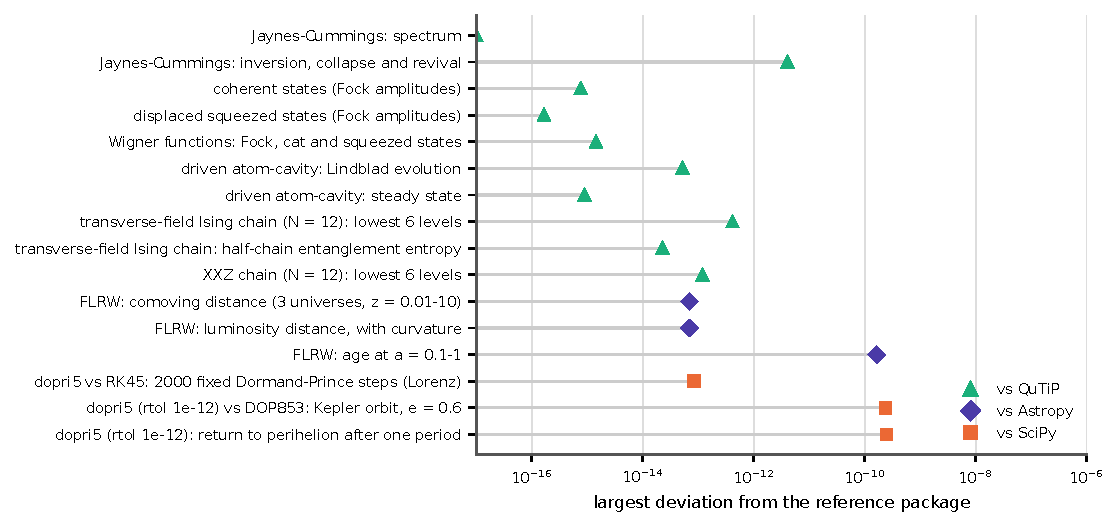
\includegraphics[width=0.85\textwidth]{fig_validation}
\caption{Largest deviation between physicskit and the reference package for
each cross-check (Table~\ref{tab:crosschecks}). The Jaynes--Cummings
spectrum agrees exactly and is drawn at the left edge. The age integral
and the two adaptive integrations are limited by their quadrature and
integration tolerances, not by round-off.}
\label{fig:validation}
\end{figure}

\begin{table}[t]
\centering\small
\caption{Cross-checks of physicskit \physicskitversion{} against QuTiP,
Astropy and SciPy (NumPy \numpyversion, SciPy \scipyversion). Each
deviation is the largest absolute difference over all times, states, grid
points or levels, relative for the cosmological quantities and for the
fixed-step integration. Each is asserted by
\code{paper/validation/run\_all.py}.}
\label{tab:crosschecks}
\begin{tabular}{llr}
\toprule
Reference & Quantity & Largest deviation \\
\midrule
\rows{tables/crosschecks}
\bottomrule
\end{tabular}
\end{table}

Thirteen of the sixteen comparisons agree to within $5\times10^{-12}$
(Fig.~\ref{fig:validation}, Table~\ref{tab:crosschecks}). The remaining
three, the age of the universe and the two adaptive integrations, agree to
$3\times10^{-10}$, which is the accuracy their tolerances request.

\paragraph{Against closed-form results.} Table~\ref{tab:analytic} lists
results that gallery examples reproduce and assert, two or three per
domain. Among them are the zeros of the Lane--Emden functions, the
figure-eight choreography, Lyapunov spectra, the Bethe ansatz, TKNN Chern
numbers, the Casimir energy, the Blasius boundary layer, Jaynes--Cummings
vacuum Rabi oscillations, Landau damping, the Dirac fine structure, the
deflection of starlight, Kerr ISCO radii, the semicircle and
Marchenko--Pastur laws, and the Onsager--Yang magnetization. The validation
script re-runs each of these examples; the whole validation takes about
30 seconds.

\begin{table}[p]
\centering\scriptsize
\caption{Closed-form and literature results asserted by the gallery
examples (folder \code{examples/}), with the tolerance of each assert;
where an example asserts two results, both tolerances are given. KS:
Kolmogorov--Smirnov.}
\label{tab:analytic}
\begin{tabularx}{\textwidth}{>{\raggedright\arraybackslash}X>{\raggedright\arraybackslash}p{3.6cm}>{\raggedright\arraybackslash}p{4.2cm}>{\raggedright\arraybackslash}p{1.7cm}}
\toprule
Result & Reference & Example & Tolerance \\
\midrule
\rows{tables/analytic}
\bottomrule
\end{tabularx}
\end{table}

%----------------------------------------------------------------------------
\section{Performance}
\label{sec:performance}

\begin{figure}[t]
\centering
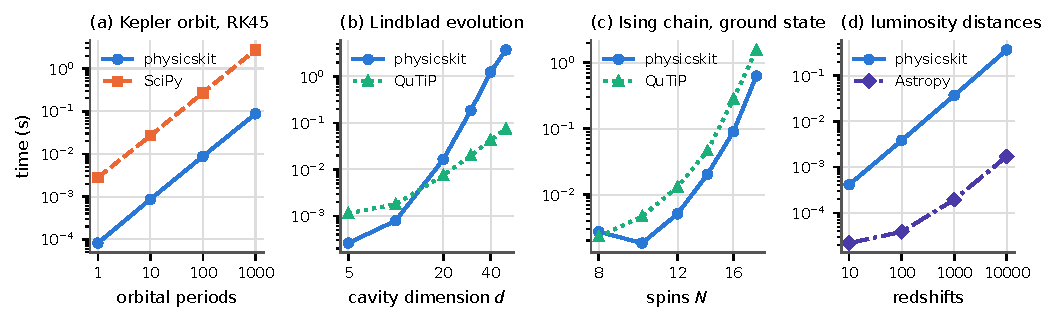
\includegraphics[width=\textwidth]{fig_benchmarks}
\caption{Wall-clock time on one thread, best of three calls after a
warm-up call. (a)~An eccentric Kepler orbit over many periods with the
adaptive Dormand--Prince integrator at the same tolerances, physicskit
(numba) against SciPy's \code{solve\_ivp}. (b)~Lindblad evolution of a
driven, damped cavity of dimension $d$, 101 output times, physicskit
(Liouvillian exponential) against QuTiP's \code{mesolve}. (c)~The two
lowest levels of a transverse-field Ising chain of $N$ spins, from
building the Hamiltonian to the sparse eigensolver. (d)~Luminosity
distances at $n$ redshifts. The packages give the same results at every
size.}
\label{fig:benchmarks}
\end{figure}

We run each case in a fresh process with one BLAS thread, on an Apple M4
laptop (\benchplatform). Each case is called once before it is timed, so
that numba compilation and the set-up of QuTiP and Astropy are not
counted, and we report the best of three calls
(Fig.~\ref{fig:benchmarks}, Table~\ref{tab:bench}).

\begin{table}[t]
\centering\small
\caption{Time (s) on one thread, at the smallest and largest size of each
task, and the ratio of the reference package's time to physicskit's
(above 1: physicskit is faster).}
\label{tab:bench}
\begin{tabular}{llrlrr}
\toprule
Task & Size & physicskit & Reference & time & ratio \\
\midrule
\rows{tables/bench}
\bottomrule
\end{tabular}
\end{table}

The results show where each design pays off. For ODEs, physicskit's
compiled integrator is about 30 times faster than SciPy's \code{solve\_ivp}
on the same tableau and tolerances, because its right-hand side is called
from compiled code rather than from the Python interpreter
[Fig.~\ref{fig:benchmarks}(a)]. For spin chains, building the Hamiltonian
directly in the bit basis is 2.5 times faster than QuTiP's tensor products
at 18 spins [Fig.~\ref{fig:benchmarks}(c)]. For open systems, physicskit's
exponential of the Liouvillian is exact up to round-off and faster for
small systems, but its cost grows as $d^6$; QuTiP's ODE integration
overtakes it between $d = 10$ and $d = 20$ and is 50 times faster at $d = 50$
[Fig.~\ref{fig:benchmarks}(b)]. For cosmological distances, Astropy's
vectorized integrals are 20 to 200 times faster than physicskit's
quadrature, which evaluates one redshift at a time
[Fig.~\ref{fig:benchmarks}(d)]. For open systems beyond a few hundred
states and for cosmology in production, QuTiP and Astropy are the right
tools. physicskit's choices favour code that a student can read and that
is exact where exactness is cheap.

%----------------------------------------------------------------------------
\section{Teaching}
\label{sec:teaching}

physicskit was written to be read as well as used. Its gallery holds 392
examples across the fourteen domains, each a short script, downloadable as
a Python file or a Jupyter notebook, that explains its physics and checks
it. Nineteen long-form tutorials, among them a guide to each domain's units
and conventions, go deeper. Each domain also has a history page that tells
its field as a chronology of breakthroughs, over 300 in all, from Kepler and Newton to
GW150914, from Planck to tensor networks, and from Wigner's semicircle to
the SYK model. Every breakthrough links to its own gallery examples, whose
titles name it, and no example is shared between two breakthroughs, so a
reader can go from a date in the history of physics to code that
reproduces the result. Because every example asserts what it shows, the
history pages cannot drift from what the code does.

%----------------------------------------------------------------------------
\section{Availability and outlook}
\label{sec:outlook}

physicskit is distributed on PyPI (\code{pip install physicskit}) under the
MIT license, and this release is archived on Zenodo~\cite{physicskit}. It
requires NumPy, SciPy, matplotlib, numba, SymPy, Plotly and tqdm;
pint and h5py are optional, for unit interoperability and HDF5 output.
Its source, documentation and coverage report are at
\url{https://github.com/cpoli/physicskit} and
\url{https://cpoli.github.io/physicskit}. Every script behind this paper,
from validation and benchmarks to figures and listings, is in the
\code{paper/} directory of the repository. physicskit belongs to a family
of packages with the same architecture and history-driven documentation,
with mathematicskit, chemistrykit and the tight-binding package
tbkit~\cite{tbkit}.

The roadmap of the project measures progress not by feature parity with
research codes but by whether each domain covers the canonical topics of a
course in its field, tells their history, and checks every example. The
benchmarks of Sec.~\ref{sec:performance} point to two extensions within
that scope: Krylov propagation of the Lindblad equation for larger open
systems, and vectorized cosmological distances.

\section*{Acknowledgements}
% TODO: acknowledgements and funding.

\bibliographystyle{unsrt}
\bibliography{references}

\end{document}
